% Entity-relationship diagram of the repair knowledge-base data model:
% REPAIR_ENTRY linked to SUBSYSTEM, PART, SERVICE_TICKET and CAPA_CASE.
\documentclass{article}
\usepackage[paperwidth=120cm,paperheight=120cm,margin=10mm]{geometry}
\pagestyle{empty}
\providecommand{\babelsublr}[1]{#1}
\usepackage{tikz}
\usepackage{pgfplots}
\pgfplotsset{compat=1.18}
\usetikzlibrary{arrows.meta, positioning, shapes.geometric, shapes.misc, calc, fit, backgrounds, decorations.pathmorphing, patterns, angles, quotes}
\begin{document}
\babelsublr{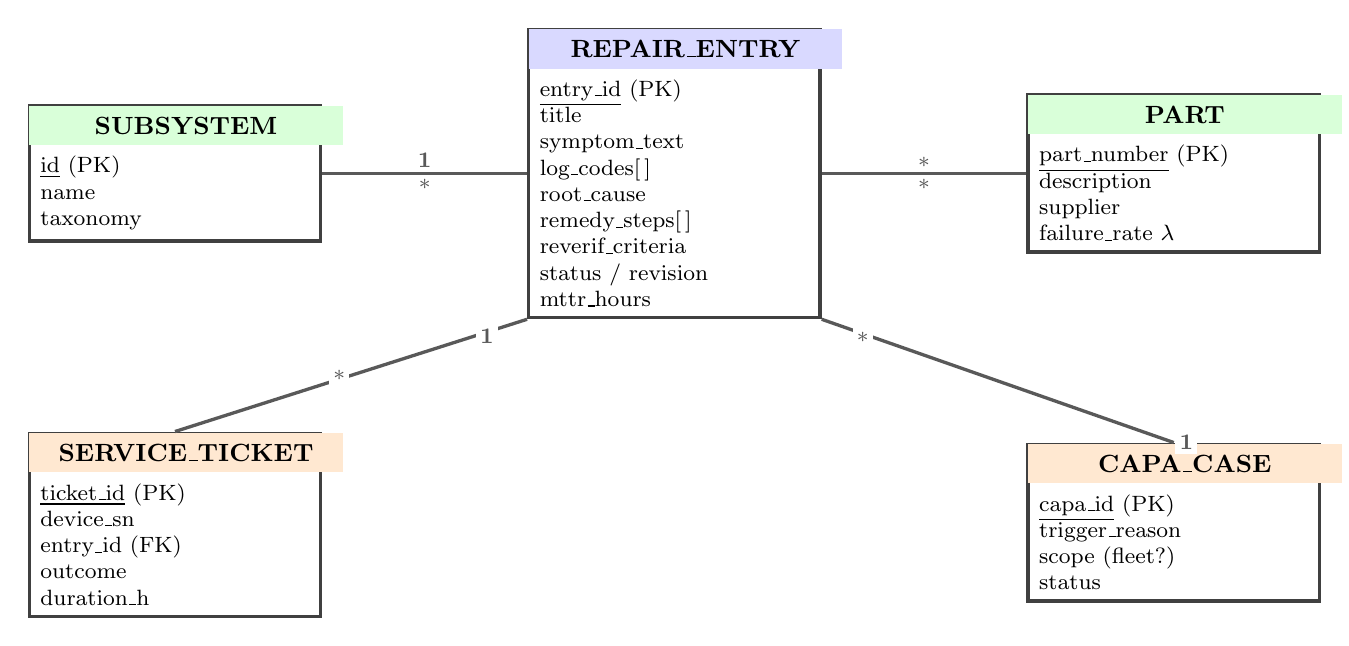
\begin{tikzpicture}[>=Stealth, font=\small,
    entity/.style={rectangle, draw=black!75, very thick, inner sep=0pt,
      text width=3.7cm},
    title/.style={fill=blue!15, inner sep=4pt, align=center, text width=3.7cm,
      font=\bfseries\small},
    title2/.style={fill=green!15, inner sep=4pt, align=center, text width=3.7cm,
      font=\bfseries\small},
    titlec/.style={fill=orange!18, inner sep=4pt, align=center, text width=3.7cm,
      font=\bfseries\small},
    fields/.style={inner sep=4pt, align=left, text width=3.7cm, font=\footnotesize},
    rel/.style={very thick, black!65},
    card/.style={font=\footnotesize\bfseries, fill=white, inner sep=1.5pt}]

  % central entity: REPAIR_ENTRY
  \node[entity] (re) at (0,0) {
    \tikz\node[title]{REPAIR\_ENTRY};\\[-1pt]
    \tikz\node[fields]{%
      \underline{entry\_id} (PK)\\
      title\\
      symptom\_text\\
      log\_codes[\,]\\
      root\_cause\\
      remedy\_steps[\,]\\
      reverif\_criteria\\
      status / revision\\
      mttr\_hours};
  };

  % SUBSYSTEM (left)
  \node[entity, left=2.6cm of re] (sub) {
    \tikz\node[title2]{SUBSYSTEM};\\[-1pt]
    \tikz\node[fields]{%
      \underline{id} (PK)\\
      name\\
      taxonomy};
  };

  % PART (right)
  \node[entity, right=2.6cm of re] (part) {
    \tikz\node[title2]{PART};\\[-1pt]
    \tikz\node[fields]{%
      \underline{part\_number} (PK)\\
      description\\
      supplier\\
      failure\_rate $\lambda$};
  };

  % SERVICE_TICKET (below-left)
  \node[entity, below=2.4cm of sub] (tick) {
    \tikz\node[titlec]{SERVICE\_TICKET};\\[-1pt]
    \tikz\node[fields]{%
      \underline{ticket\_id} (PK)\\
      device\_sn\\
      entry\_id (FK)\\
      outcome\\
      duration\_h};
  };

  % CAPA_CASE (below-right)
  \node[entity, below=2.4cm of part] (capa) {
    \tikz\node[titlec]{CAPA\_CASE};\\[-1pt]
    \tikz\node[fields]{%
      \underline{capa\_id} (PK)\\
      trigger\_reason\\
      scope (fleet?)\\
      status};
  };

  % relationships with cardinalities
  \draw[rel] (sub.east) -- node[card, above]{1} node[card, below]{$*$} (re.west);
  \draw[rel] (re.east) -- node[card, above]{$*$} node[card, below]{$*$} (part.west);
  \draw[rel] (tick.north) -- node[card, left]{$*$} (re.south west)
     node[card, pos=0.85, right]{1};
  \draw[rel] (re.south east) -- node[card, pos=0.15, left]{$*$} (capa.north)
     node[card, right]{1};

\end{tikzpicture}}
\end{document}
